\subsubsection{\stid{4.14} VeloC: Very Low Overhead Checkpointing System}

\paragraph{Overview.}
The VeloC-SZ project aims to provide VeloC, a high-performance,
scalable checkpoint/restart framework that leverages multi-level
checkpointing (the combination of several resilience strategies and
heterogeneous storage) to ensure that ECP applications run to
completion with minimal performance overhead. It delivers a
production-ready solution that increases development productivity by
reducing the complexity of having to deal with a heterogeneous storage
stack and multiple vendor APIs. VeloC offers a client library that can
be used by the applications to capture local application states, which
are then coordinated and persisted using a resilience engine.  VeloC
runs the resilience engine asynchronously, which overlaps a large part
of the checkpointing with the application runtime, thereby reducing
its overhead. An overview of the architecture of VeloC is depicted
in Figure~\ref{fig:veloc:arch}.

VeloC has been released and shows significant lower checkpointing
overhead for several ECP applications, such as HACC, LatticeQCD,
EXAALT.

\paragraph{Key Challenges.}
VeloC addresses several key challenges:
\vspace{-1em}

\paragraph{\emph{I/O bottlenecks:}} applications typically employ
simple checkpoint-restart mechanisms to survive failures that directly
use a parallel file system. With diminishing I/O bandwidth available
per core, this leads to high checkpointing overhead and is not
sustainable.
\vspace{-1em}

\paragraph{\emph{Deep heterogeneous storage:}} To compensate for
diminishing parallel file system I/O bandwidth per core, the storage
stack is becoming increasingly deeper and heterogeneous: node-local
NVRAM, burst buffers, key-value stores, etc. However, the variety of
vendor APIs and performance characteristics make it difficult for
application developers to take advantage of it.
\vspace{-1em}

\paragraph{\emph{Restart-in-place:}} a majority of failures affect
only a small part of the nodes where the job is running. Therefore,
reusing the surviving nodes to restart from the latest checkpoint
immediately after a failure is more efficient than submitting a new job,
which may wait for a long time in the batch queue.
\vspace{-1em}

\paragraph{\emph{Efficient serialization:}} The critical data structures
of HPC applications that need to be checkpointed are constantly
growing in size and complexity. Manual serialization of such data
structures as contiguous sequences of bytes to be written into
checkpoints is both tedious (leading to loss of productivity) and
inefficient (leading to longer runtime). Therefore, automated
optimized serialization support is needed.

\paragraph{Solution Strategy}

To address these challenges, VeloC adopts the following principles:
\vspace{-1em}

\paragraph{\emph{Multi-level checkpointing:}} is based on the idea
that a majority of failures can be mitigated without involving the
parallel file system: node-local checkpoints can be used to recover
from software bugs, replication/erasure coding can be used to recover
from most combinations of node failures. This reduces the frequency of
checkpointing to the parallel file system and therefore the I/O
bottlenecks.
\vspace{-1em}

\paragraph{\emph{Asynchronous mode:}} once a node-local checkpoint has
been written, applications do not need to wait for replication,
erasure coding or writes to the parallel file system: these can be
applied in the background, while the application continues
running. However, in this case, it is important to minimize
interference with the application execution.
\vspace{-1em}

\paragraph{\emph{Transparent use of heterogeneous storage:}} we
developed several techniques that can leverage a variety of local
storage (in-memory file systems, flash storage) and external storage
(burst buffers, key-value stores, parallel file systems)
options. These techniques select the best available storage options,
tune them with the optimal parameters and leverage any vendor-specific
API if needed to transfer data.
\vspace{-1em}

\paragraph{\emph{Job scheduler integration:}} to implement
restart-in-place, we have developed a series of scripts that interact
with a variety of job schedulers to run jobs with spare nodes,
continue execution on failures, restart on the surviving nodes and
spares using the fastest possible recovery strategy (which ideally
avoids reading checkpoints from the parallel file system). This is
transparent to the users.
\vspace{-1em}

\paragraph{\emph{Declarative API and automated serialization:}} we
offer a simple API that enables users to either manually capture
checkpoints into files or to define memory regions that are
automatically serialized into checkpoint files.
\vspace{-1em}

\paragraph{\emph{Modular design:}} applications link with a client
library that is responsible to manage local checkpoints, while a
separate engine is responsible to employ the rest of the resilience
strategies as plugable modules. This simplifies the implementation
of the asynchronous mode, it enables users the flexibility to choose any
combination of resilience strategies, as well as, to customize their
checkpointing pipeline (e.g., add new post-processing operations such
as analytics or compression).

\paragraph{Recent Progress}

We met and closely collaborated with several ECP application teams in
an effort to address their checkpointing needs. Most of our current
efforts involve the HACC, LatticeQCD, and EXAALT teams. We also
started integrating VELOC into NWChemEX. Based on feedback from
several teams, we extended VELOC to support multiple communication
protocols that reduce dependencies on external libraries (such as
Boost) if desired.  Furthermore, we added preliminary support for
checkpoint aggregation, which reduces the number of checkpoint files
from one per rank to a desired smaller number.

\begin{wrapfigure}{l}{0.47\textwidth}
  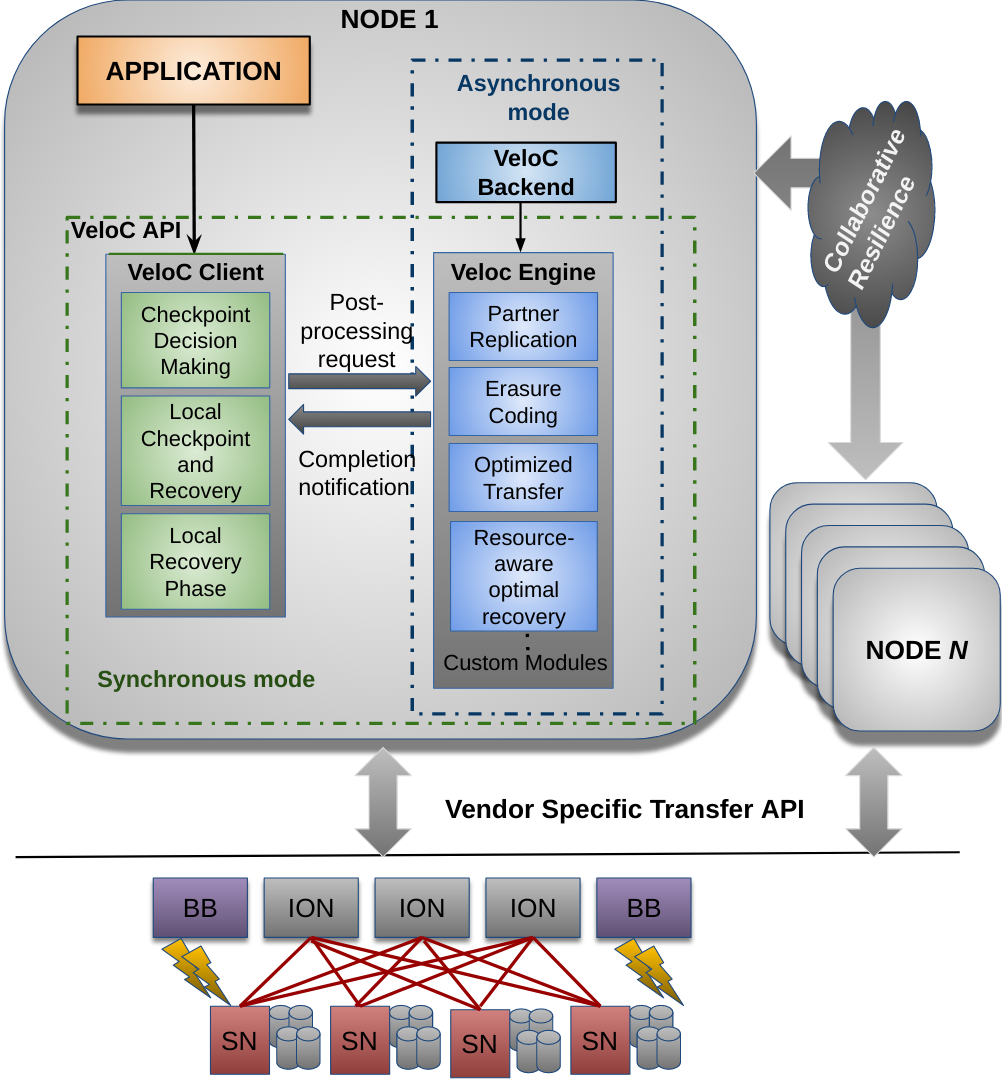
\includegraphics[width=0.4\textwidth]{projects/2.3.4-DataViz/2.3.4.14-VeloC-SZ/veloc-arch}
  \caption{VeloC: Architecture}%
  \label{fig:veloc:arch}%
\end{wrapfigure}

In terms of capabilities, we refactored the VELOC code to abstract all
interactions with external storage in the code, which allows flexible
support to persist checkpoints on a variety of options in addition to
conventional POSIX-based parallel file systems. In particular, to
illustrate this capability, we added support for DAOS, an object-based
store developed by Intel and planned to be used by the Aurora
supercomputer. This paves the way to include support for other
object-based and persistent key-value stores, likely to become popular
in the future and developed by the vendors and/or the HPC community.

Second, we continued our efforts to provide an incremental
checkpointing capability in VELOC for HPC applications that need to
checkpoint data structures that change only partially between the
checkpoint requests.  Our proposal is exploring hash-based
de-duplication to optimize the trade-off between reducing checkpoint
sizes at the expense of identifying and consolidating the increments
in a heterogeneous environment (GPU + CPU).  This has two advantages:
(1) it produces smaller checkpoints, which saves storage space across
the whole heterogenous storage stack; (2) it improves checkpointing
performance by reducing the data transfer overheads, which impact both
the blocking phase and the asynchronous operations.

Third, we continued working on the checkpoint aggregation, which allows
N local files produced during the blocking phase of VELOC to be aggregated
asynchornously into M files on the external storage. Since state of
art aggregation approaches (e.g. MPI-IO) are designed for collective
blocking I/O, we developed our own algorithms to enable asynchronous
aggregation. In particular, we proposed a decoupled peer-to-peer
leader election algorithm that allows independent groups of (potentially
remote) ranks to consolidate their data on a single rank, which is then
responsible to write a single file to the PFS.

\paragraph{Testing, Continuous Integration, and Experience on Early Access Systems}
We continued working towards new features that facilitate better
integration with the ECP ecosystem. We extended the test suite of
VELOC (runnable both independently and with continuous integration) to
include more comprehensive set of combinations of scenarios, both for
VELOC and its subcomponents. In particular, we added support for
testing the refactored VELOC code that allows multiple options for
external storage and its new DAOS support. Furthermore, we
experimented with VELOC at small scale on various early testbeds
encouraged for use by the ECP community. Notably, we experimented on
Spock, a proxy to Frontier hosted at ORNL. From the VELOC perspective,
it features both high performance memories and local storage
(NVMe-based SSD), while persistent storage is provided through a PFS
mount point. Despite the instability of the software stack on this
testbed, we successfully tested VELOC with the standard battery of
tests and confirmed its correctness at small scale. Presque (ANL) is
another platform we targeted as it provides access to a DAOS
deployment. We were successful in running the refactored version of
VELOC to checkpoint small data sizes, but encountered issues with DAOS
(reported to Intel) when using larger checkpoint sizes.

\paragraph{Next Steps}
We are working towards several goals: (1) refine incremental
checkpointing techniques; (2) refine asynchronous checkpoint
aggregation techniques; (3) continue hardening the integration with
existing ECP applications; (4) test VELOC on more ECP testbeds, in
particular CRUSHER. In parallel, we will continue the collaboration
with the ECP application teams to address new requirements as they
arise.
